\documentclass{article}%
\usepackage[T1]{fontenc}%
\usepackage[utf8]{inputenc}%
\usepackage{lmodern}%
\usepackage{textcomp}%
\usepackage{lastpage}%
\usepackage[head=40pt,margin=0.5in,bottom=0.6in]{geometry}%
\usepackage{graphicx}%
%
\title{\textbf{Jubilados y pensionados de la Cantv protestan por tablas salariales}}%
\author{El Nacional Web}%
\date{16/10/2018}%
%
\begin{document}%
\normalsize%
\maketitle%
\textbf{URL: }%
http://www.el{-}nacional.com/noticias/protestas/jubilados{-}pensionados{-}cantv{-}protestan{-}por{-}tablas{-}salariales\_255950\newline%
%
\textbf{Periodico: }%
EN, %
ID: %
255950, %
Seccion: %
Protestas\newline%
%
\textbf{Palabras Claves: }%
Economía, Gobierno, Cantv\newline%
%
\textbf{Derecho: }%
2.3%
, Otros Derechos: %
NO\_TIENE%
, Sub Derechos: %
2.3.4%
\newline%
%
\textbf{EP: }%
SI\newline%
\newline%
%
\textbf{\textit{La avenida Libertador está trancada por los trabajadores. La PNB se encuentra en el lugar}}%
\newline%
\newline%
%
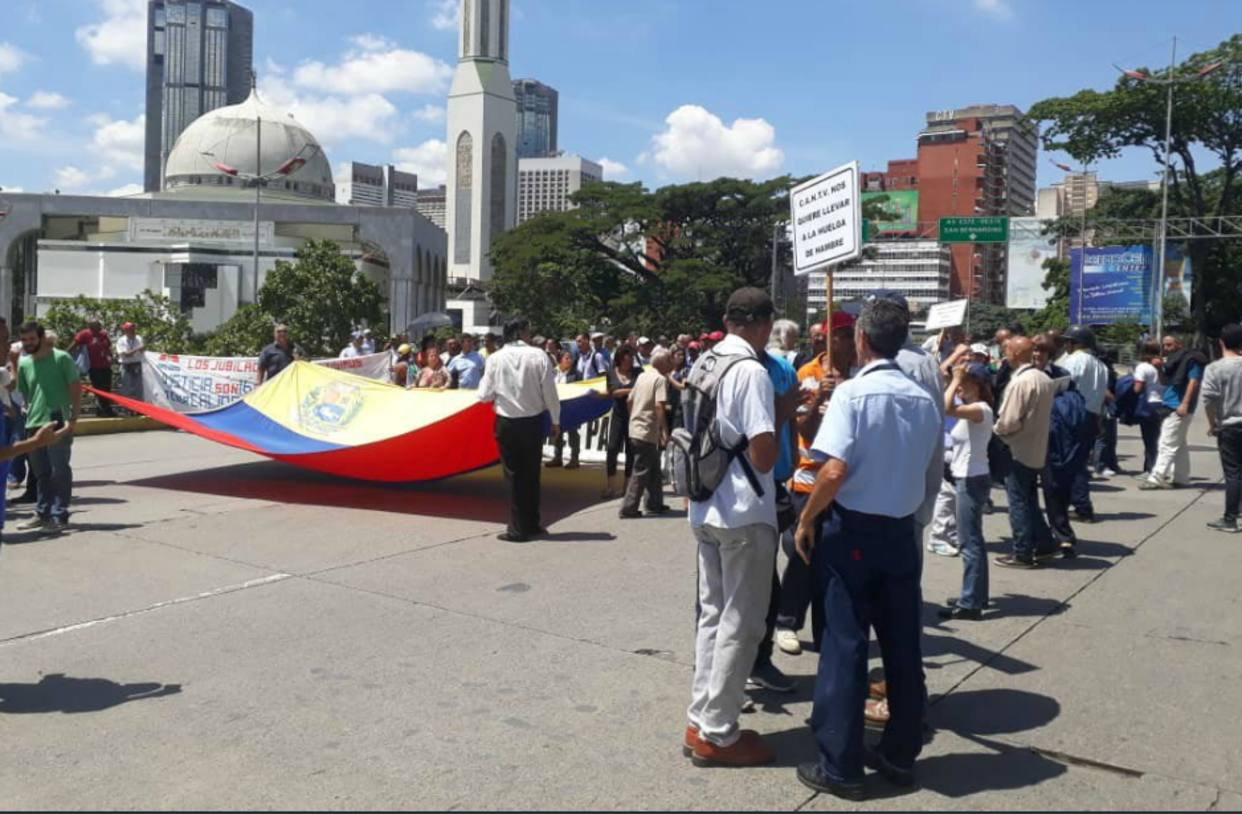
\includegraphics[width=300px]{178.jpg}%
\newline%
%
Trabajadores jubilados y pensionados de la Compañía Anónima Nacional Teléfonos de Venezuela (Cantv) protestan este martes en la avenida Libertador de Caracas para exigir respeto a las tablas salariales.%
\newline%
%
Reportes de Twitter indican que la arteria vial está trancada. Usuarios sugieren tomar previsiones a los conductores.~Funcionarios de la Policía Nacional Bolivariana (PNB) se encuentran en el lugar.%
\newline%
%
Juan Véliz, presidente del Sindicato de la Cantv, informó que este 17 de septiembre tendrán~una actividad en la Plaza de la Moneda con los trabajadores del IVSS.%
\newline%
%
Un jubilado de la compañía telefónica manifestó que su pensión no se iguala a las de los trabajadores activos.%
\newline%
%
\end{document}